\documentclass[pdftex,12pt,letter]{article}
\usepackage{fancyhdr}
\usepackage{enumerate}
\usepackage{tabularx}
\usepackage{graphicx}
\usepackage{array}
\usepackage[toc,page]{appendix}
\usepackage[justification=justified,singlelinecheck=false]{caption}
\usepackage{placeins}
\pagestyle{fancy}
\makeatletter
  \renewcommand\@seccntformat[1]{\csname the#1\endcsname.\quad}
\makeatother

\newcolumntype {Y}{ >{\raggedright \arraybackslash }X}
\newcommand{\HRule}{\rule{\linewidth}{0.5mm}}
\captionsetup{labelformat=empty}

\begin{document}

\begin{titlepage}
\begin{flushright}
\HRule \\[0.4cm]
{ \bfseries
{\huge EECS 395 Project Proposal\\[1cm]}
{\Large for\\[1cm]}
{\huge Chocolate Box\large\\[.1cm]
A Procedural Level Generator for Unity\\[3cm]}
{\large Prepared by\\[1cm]James Fitzpatrick\\Stuart Long\\Frank Singel\\[2cm]
Version 1.0\\
February 3, 2014\\
}}
\end{flushright}
\end{titlepage}
\begin{table}[!h]
\caption*{\bfseries Revision History}
\begin{tabularx}{\textwidth }[t]{|l|l|Y|l|}
\hline
\bfseries Name & \bfseries Date & \bfseries Reasons for Change & \bfseries Version \\ \hline
\end{tabularx}
\end{table}
\FloatBarrier
\newpage
\section{Abstract}
\textit{Chocolate Box} will be a helpful tool for video game developers. Its goal is to provide an easy-to-use software library for any game developers working with the common game engine, Unity. It will allow developers to create unique levels purposed towards whatever game they are currently developing. These levels will be pseudo-random, so each level created will be unique. This tool will enable developers to create games with an infinite variety of levels which is perfect for arcade-like games. 
\\\\
\textit{Chocolate Box} will be built for 2-dimensional side-scrolling platformers, similar to classic games such as \textit{Super Mario Bros} and \textit{Megaman}. Users will be able to specify constraints and parameters on this library to mold the generated levels to fit their needs. 
\\\\
This system will be composed of a series of Unity scripts which users will interact with through the default Unity interface. The main issues involved in this project will be generating levels that are playable, fun, and fit developers' desires.
\newpage

\section{Introduction}
\subsection{Relevant Background}
Unity 4.3 was released a few short months ago in late 2013. One the major new features introduced was full support for 2D games. Before this new version, Unity had been intended as a game engined for 3D games, with any support for 2D having to come from unofficial and unsupported third parties. Given its recent introduction, there are currently not many libraries created for use with Unity's new 2D framework. Thus \textit{Chocolate Box} would be one of the first and it is certain that nothing like \textit{Chocolate Box} currently exists. Procedural level generation is both a challenging problem and a useful tool. In can be seen in modern games today such as \textit{Minecraft}, \textit{Terraria}, and \textit{Spelunky}. It allows games to provide an infinite variety of experiences for their players which keeps games interesting and long-lasting.
\subsection{Project Description}
\textit{Chocolate Box} will be a Unity asset that procedurally generates levels at runtime. Unity game developers will be able to incorporate this asset into their game scenes, allowing their games to have procedurally generated levels that smoothly integrate with their game's theme and the rest of their game. Procedurally generating a game level has many challenges associated with it. In brief, this problem encompasses determining a unique level layout and ensuring that layout is playable, fun, and constrains to user constraints. Users will use \textit{Chocolate Box} via a single Unity script. Therefore, they will interact with it via the Unity interface, specifically the Inspector.
\subsection{Related Work}
There currently does not exist any form of library to provide procedural level generation for Unity in either a 2D or 3D form. However, procedural level generation has been done for games such as \textit{Minecraft}. Such games are not open sourced and were not developed through Unity. 
\\\\
Two of the members of the \textit{Chocolate Box} team have experience with Unity. Stuart Long helped developed a fully functional game, \textit{Gumdrop Gauntlet}, in Unity. WHAT DID JAMES DO?!?! Frank Singel has the most experience on the team in the area of AI which will prove useful when creating the generation algorithms.
\subsection{Goals}
Below is described in detail the full feature set of \textit{Chocolate Box}, the team's methodology in developing it, and this project's software requirements. By the end of February, a month from now, the team expects to be able to generate a rudimentary level and to spawn enemies in it in a rudimentary fashion.
\section{Application}
\section{Methodology}
\section{Software Design}
\section{Project Management}
The \textit{Chocolate Box} team is small and familiar, allowing for a more project management schema. Stuart Long is the project manager and he will be responsible for the overall project management. Each member of the team will have set responsibilities, but the team as a whole will collaborate on any challenges or problems that arise if need be. The team will be using the on-line task tracking system Trello to keep track of project tasks and bugs. A private git repository on GitHub has been secured to use as the version control system for the project. Below is a Gantt chart outlining the broad goals and time-line of the project that the team have so far determined.
\centerline{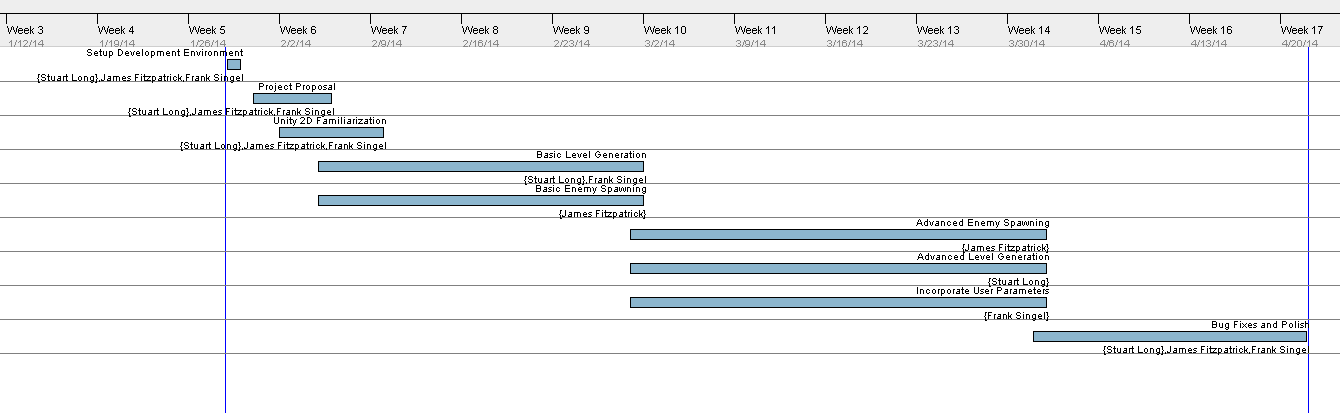
\includegraphics[width=7in]{GanttSS.png}}
\FloatBarrier
\section{User Interface}
\textit{Chocolate Box} will be fully integrated into Unity. Thus it will not requires its own User Interface. Instead, it will be used through Unity's own interface, specifically the part known as the Inspector. A mock up of this interface can be seen on the right-hand side of the figure below.

\centerline{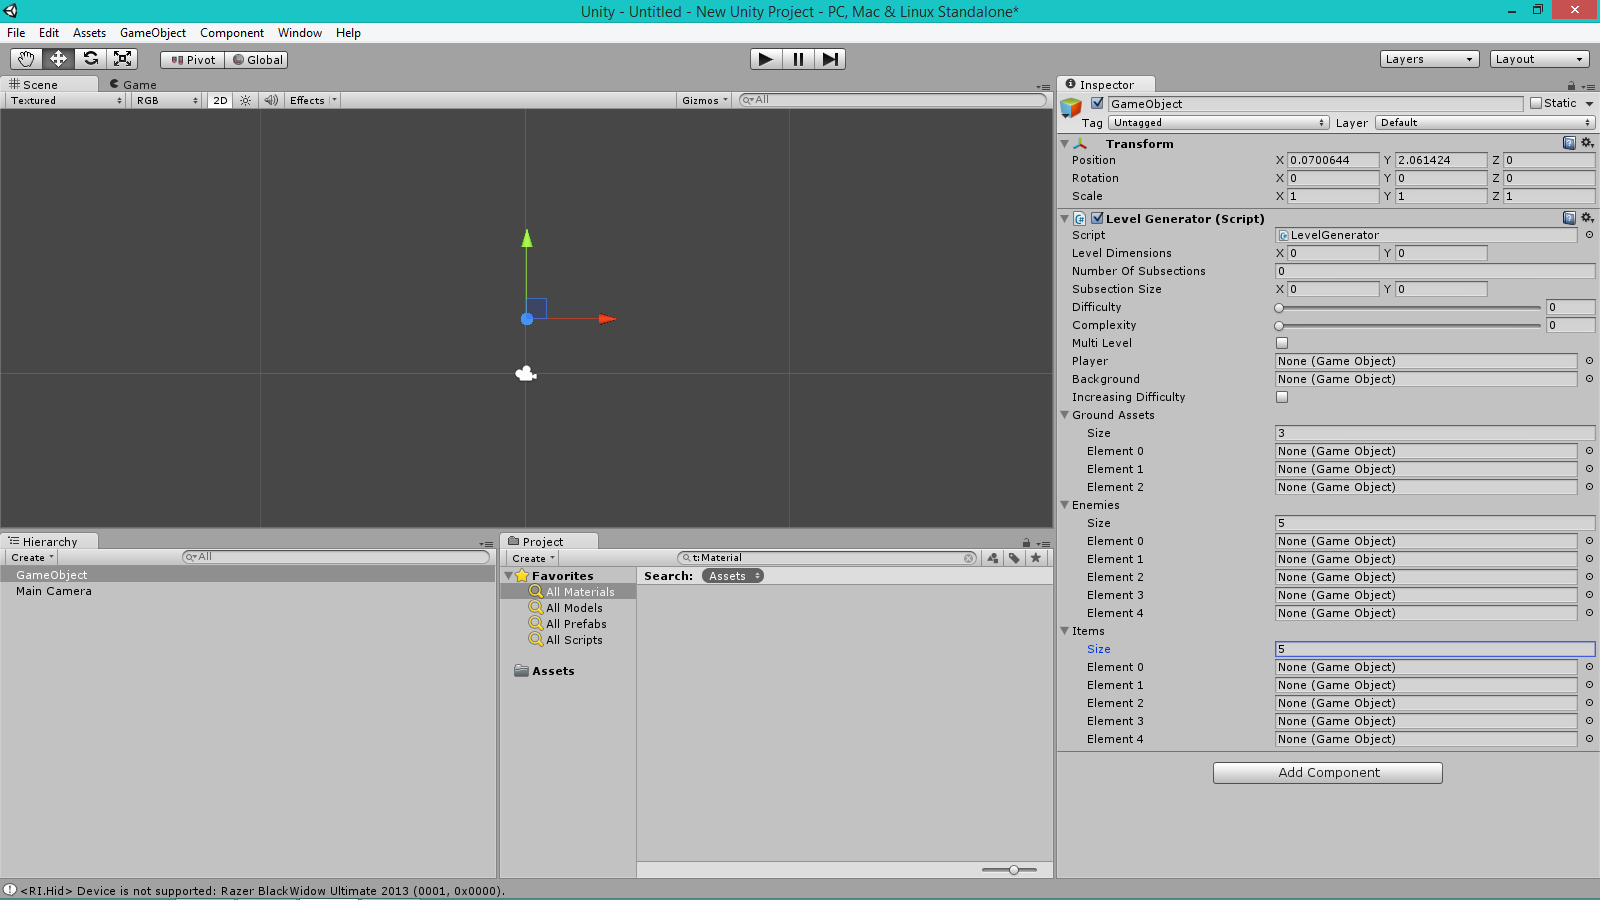
\includegraphics[width=7in]{UnitySS.png}}
\FloatBarrier
\end{document}